\documentclass[12pt,convert={density=150}]{standalone}

\usepackage{amsmath}
\usepackage{amsfonts}
\usepackage{amssymb}
\usepackage{fontspec}
\usepackage{tikz}

\usetikzlibrary{arrows}
\usetikzlibrary{decorations.markings}
\usetikzlibrary{decorations.text}
\usetikzlibrary{positioning}

\definecolor{myblue}{RGB}{38,120,179}

\begin{document}
\footnotesize
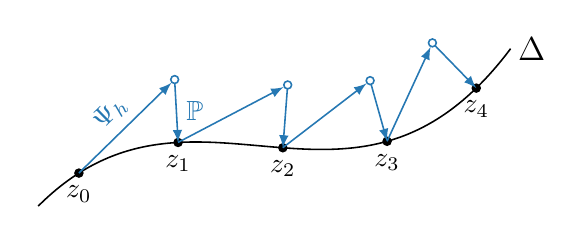
\begin{tikzpicture}[yscale=1.3333, xscale=1.3333,
    decoration={
        markings,
		mark=at position 0.1 with \coordinate (M1);,
		mark=at position 0.3 with \coordinate (M2);,
		mark=at position 0.5 with \coordinate (M3);,
		mark=at position 0.7 with \coordinate (M4);,
		mark=at position 0.9 with \coordinate (M5);,
        mark={ between positions 0.1 and 0.9 step 0.2 with {
        			\node[circle, draw=black, fill=black, inner sep=1pt] {};
        	 }
        },
        mark=at position 0.3 with {
            		\draw[myblue, line width=0.2mm, latex-] (0,0mm) -- (0,8mm) node [midway, right, rotate=270, sloped] {$\mathbb{P}$};},
        mark={ between positions 0.5 and 0.9 step 0.2 with {
            		\draw[myblue, line width=0.2mm, latex-] (0,0mm) -- (0,8mm);
		     }
        },
		mark=at position 0.3 with { \node (P2) at (0,8mm) [circle, draw=myblue, fill=white, inner sep=1pt] {};},
		mark=at position 0.5 with { \node (P3) at (0,8mm) [circle, draw=myblue, fill=white, inner sep=1pt] {};},
		mark=at position 0.7 with { \node (P4) at (0,8mm) [circle, draw=myblue, fill=white, inner sep=1pt] {};},
		mark=at position 0.9 with { \node (P5) at (0,8mm) [circle, draw=myblue, fill=white, inner sep=1pt] {};},
    }]

	\clip (0.4,2.4) rectangle (5.4,4.2);
	
	\draw[black, line width=0.2mm, postaction=decorate] (0.5,2.5) .. controls(2,4) and (3.5,2) .. (5,4);
	
	\node[black] (Delta) at (5.2,4) {\large$\Delta$};
	
	\draw[myblue, line width=0.2mm, -latex] (M1) -- (P2) node [midway, above, sloped] {$\Psi_{h}$};
	\draw[myblue, line width=0.2mm, -latex] (M2) -- (P3);
	\draw[myblue, line width=0.2mm, -latex] (M3) -- (P4);
	\draw[myblue, line width=0.2mm, -latex] (M4) -- (P5);
	
	\node[black] (z0) at ([shift={(0,-.2)}]M1) {$z_{0}$};
	\node[black] (z1) at ([shift={(0,-.2)}]M2) {$z_{1}$};
	\node[black] (z2) at ([shift={(0,-.2)}]M3) {$z_{2}$};
	\node[black] (z3) at ([shift={(0,-.2)}]M4) {$z_{3}$};
	\node[black] (z4) at ([shift={(0,-.2)}]M5) {$z_{4}$};
	
    \end{tikzpicture}
\end{document}
